\documentclass[a4paper,12pt]{report}
\usepackage[utf8]{inputenc}
\usepackage[T1]{fontenc}
\usepackage[french]{babel}
\usepackage{graphicx}
\usepackage{hyperref}
\usepackage{float}
\usepackage{amsmath}
\usepackage{booktabs}
\usepackage[margin=2.5cm]{geometry}
\usepackage{lmodern}
%\usepackage{microtype}
\usepackage[sfdefault]{roboto}
\usepackage{xcolor}
\hypersetup{
    colorlinks=true,
    linkcolor=blue,
    filecolor=magenta,
    urlcolor=cyan
}

\title{\textbf{Rapport de Comparaison des Performances entre MySQL et MongoDB}}
\author{\textbf{Auteur:} \textit{Votre Nom}}
\date{\textit{Décembre 2024}}

\begin{document}

\maketitle

\tableofcontents

\title{\textbf{Rapport de Comparaison des Performances entre MySQL et MongoDB}}
\author{\textbf{Auteur:} \textit{Brelot Julien}}

\begin{document}

\maketitle

\tableofcontents

\chapter{Introduction}
Ce rapport présente une étude comparative des performances entre MySQL et MongoDB, deux systèmes de gestion de bases de données (SGBD) très utilisés, en mettant l'accent sur les opérations CRUD (Create, Read, Update, Delete).\newline
L'objectif est de tester différentes configurations et scénarios d'utilisation pour analyser l'impact des index, de la réplication, et de la fragmentation sur les performances.\newline
La structure des tests, ainsi que les résultats obtenus, sont décrits en détail.

\chapter{Contexte et Objectifs}

\section{Systèmes Comparés}

\subsection{MongoDB}
MongoDB est un SGBD NoSQL orienté documents. Contrairement aux bases relationnelles, MongoDB stocke les données sous forme de documents JSON ou BSON, offrant une grande flexibilité structurelle. Ses caractéristiques principales incluent :
\begin{itemize}
    \item \textbf{Stockage orienté documents} : Les données sont regroupées en collections, chaque document étant un objet JSON avec une structure flexible.
    \item \textbf{Requêtes riches} : MongoDB prend en charge des requêtes complexes incluant des opérations d'agrégation et des jointures.
    \item \textbf{Scalabilité horizontale} : Avec la fragmentation (sharding), les données peuvent être réparties sur plusieurs nœuds.
    \item \textbf{Réplication} : MongoDB utilise des Replica Sets pour garantir la haute disponibilité et la tolérance aux pannes.
    \item \textbf{Indexation avancée} : MongoDB offre un support pour les index secondaires et composites afin d'optimiser les performances des requêtes.
\end{itemize}

\section{Étude des aspects de MongoDB}
\subsection{Comparaison des Performances des Requêtes}
MongoDB se distingue des bases relationnelles comme MySQL par sa capacité à exécuter des requêtes sur des données semi-structurées et non structurées. La comparaison des performances des requêtes révèle :
\begin{itemize}
    \item MongoDB excelle dans les scénarios où les données sont semi-structurées ou nécessitent une mise à jour fréquente de leur structure.
    \item MySQL, en revanche, est plus performant pour les requêtes transactionnelles complexes grâce à son moteur ACID robuste.
\end{itemize}
Des tests sur des collections contenant des millions de documents montrent que MongoDB est plus rapide pour des lectures non indexées, tandis que MySQL excelle lorsque des index adaptés sont en place.

\subsection{Performances avec et sans Indexation}
L'indexation est un facteur clé des performances :
\begin{itemize}
    \item \textbf{MongoDB sans indexation} : Les requêtes nécessitent un balayage complet des documents, ce qui ralentit considérablement les performances.
    \item \textbf{MongoDB avec indexation} : Les performances des lectures augmentent de façon exponentielle grâce à la réduction du nombre de documents scannés.
    \item \textbf{MySQL avec indexation} : Étant donné sa nature relationnelle, MySQL exploite efficacement les index pour optimiser les lectures et écritures.
\end{itemize}

\subsection{Impact de la Réplication et de la Fragmentation}
La réplication et la fragmentation influencent directement les performances et la tolérance aux pannes.
\paragraph{Réplication dans MongoDB :}
\begin{itemize}
    \item \textbf{Réplication primaire-secondaire} : Permet une haute disponibilité des données. Les écritures se font uniquement sur le nœud primaire, tandis que les lectures peuvent être réparties sur les nœuds secondaires.
    \item \textbf{Élections automatiques} : En cas de panne du nœud primaire, un nouveau primaire est élu parmi les secondaires, garantissant une continuité de service.
    \item \textbf{Impact sur les performances} : La latence d'écriture augmente avec un \texttt{write concern} élevé, car l'écriture doit être confirmée par plusieurs nœuds.
\end{itemize}

\paragraph{Fragmentation dans MongoDB :}

\begin{itemize}
    \item \textbf{Distribution des données} : Les documents sont répartis entre plusieurs shards, permettant de gérer efficacement de grandes volumétries.
    \item \textbf{Impact sur les performances} : La fragmentation améliore les temps de réponse pour les lectures et écritures parallèles, mais peut augmenter la complexité des requêtes agrégées.
\end{itemize}


\paragraph{Comparaison avec MySQL :}

\begin{itemize}
    \item \textbf{Réplication} : MySQL utilise un modèle maître-esclave classique, où les lectures peuvent être réparties, mais les écritures sont limitées au maître.
    \item \textbf{Fragmentation} : Disponible via MySQL Cluster, mais nécessite une configuration plus complexe comparée à MongoDB.
\end{itemize}

\chapter{Configurations des Tests}

\section{Architecture MongoDB}

\subsection{Standalone}

Un seul serveur MongoDB.
\begin{figure}[H]
    \centering
    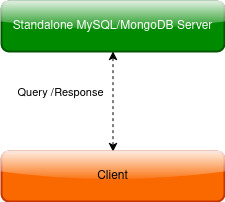
\includegraphics[width=0.8\textwidth]{architectures/Standalone.jpg}
    \caption{Architecture Standalone.}
    \label{fig:standalone}
\end{figure}

\subsection{Replica Set}

Un Replica Set avec un nœud primaire et deux nœuds secondaires.
\begin{figure}[H]
	\centering
	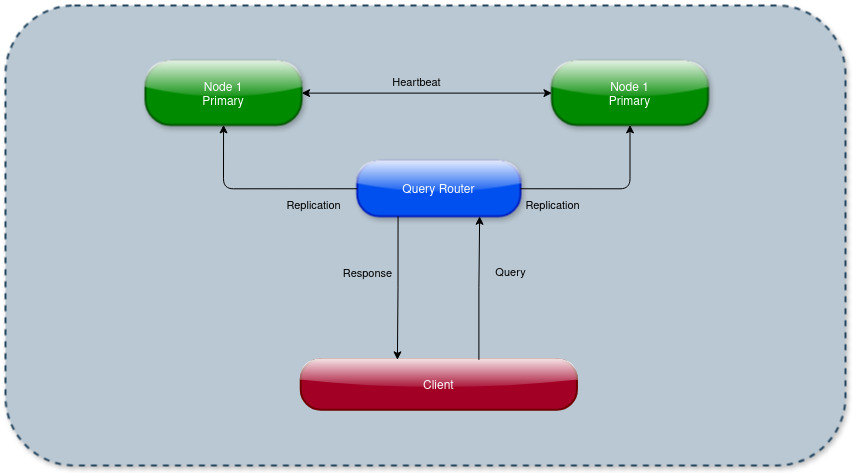
\includegraphics[width=0.8\textwidth]{architectures/MongoDBReplica.jpg}
	\caption{Architecture Replica Set.}
	\label{fig:mong-replica-set}
\end{figure}

\subsection{Sharded Cluster}
Un cluster avec trois Serveurs de configuration, un Query router, et deux shards constitués chacun de deux nœuds.

\begin{figure}
	\centering
	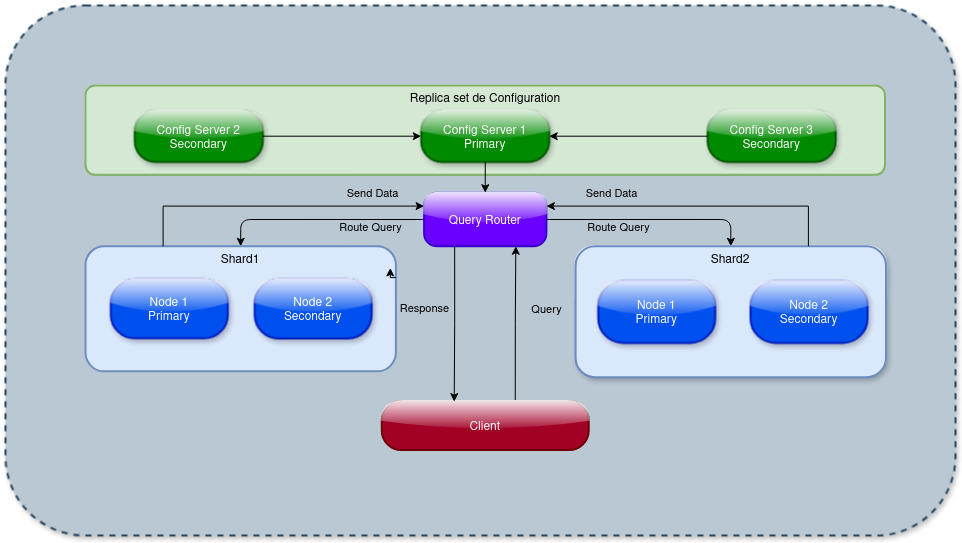
\includegraphics[width=0.8\textwidth]{architectures/MongoDBShards.jpg}
	\caption{Architecture Sharded Cluster de MongoDB.}
	\label{fig:mongo-sharded-cluster}
\end{figure}

\section{Architecture MySQL}

\subsection{Standalone}
Un serveur MySQL simple.
Voir la figure \ref{fig:standalone}.

\subsection{Sharded Architecture}

Architecture MySQL-NDB avec :
\begin{itemize}
    \item Un gestionnaire (manager).
    \item Deux nœuds de données.
    \item Un noeud SQL.
\end{itemize}

\begin{figure}[H]
	\centering
	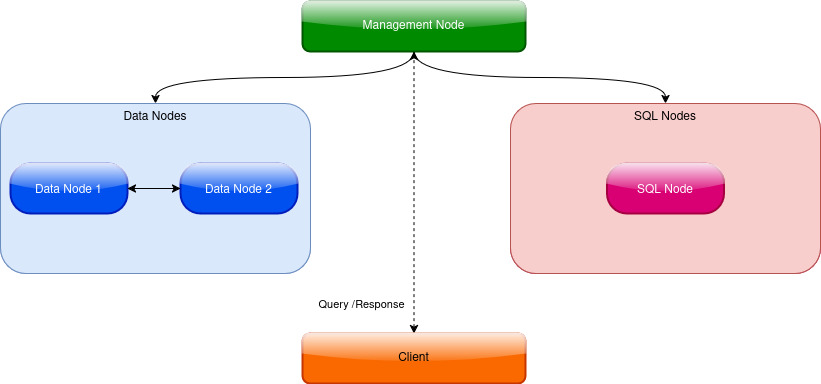
\includegraphics[width=0.8\textwidth]{architectures/MySQLCluster.jpg}
	\caption{Architecture MySQL Cluster.}
	\label{fig:mysql-cluster}
\end{figure}

\chapter{Structure des Données}
La table/collection "test" utilisée pour les tests a la structure suivante :
\begin{itemize}
    \item \textbf{id} : Identifiant unique (UUID ou auto-incrément pour MySQL, ObjectId pour MongoDB).
    \item \textbf{title} : Titre du livre (String).
    \item \textbf{author} : Auteur du livre (String).
    \item \textbf{published\_date} : Date de publication (Date).
    \item \textbf{genre} : Genre du livre (String).
    \item \textbf{price} : Prix du livre (Float).
    \item \textbf{copies\_sold} : Nombre d'exemplaires vendus (Integer).
    \item \textbf{ran} : Champ aléatoire pour les tests entre 0 et $\texttt{num\_records\_per\_many} - 1$ (Integer).
\end{itemize}
Ce qui donne pour MySQL :
\begin{verbatim}
CREATE TABLE test (
	id INT PRIMARY KEY AUTO_INCREMENT,
	title VARCHAR(255),
	author VARCHAR(255),
	published_date DATE,
	genre VARCHAR(255),
	price FLOAT,
	copies_sold INT,
	ran INT
);
\end{verbatim}

\chapter{Batterie de Tests}

\section{Types de Tests}

\begin{itemize}
    \item Tests CRUD : insertion, lecture, mise à jour, suppression.
    \item Tests avec indexation et sans indexation.
\end{itemize}

\section{Scénarios}

\begin{itemize}
    \item Opérations globales sur $\texttt{num\_records}$ données.
    \item Insertion ou mise à jour de $\texttt{num\_records\_per\_many}$ données avec variation du nombre de données initiales.
\end{itemize}

\chapter{Résultats et Analyses}

\section{Graphiques des Performances}
\begin{figure}[H]
    \centering
    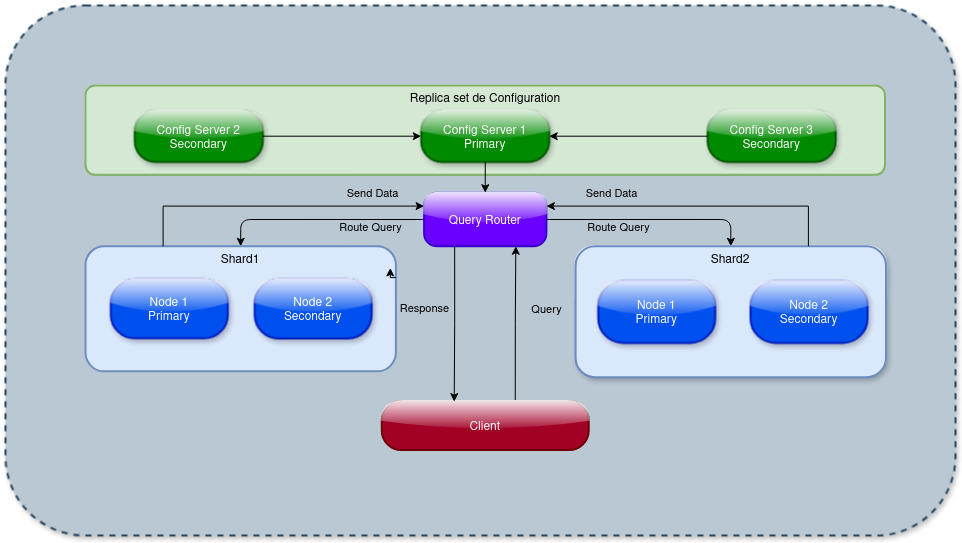
\includegraphics[width=0.8\textwidth]{architectures/MongoDBShards.jpg}
    \caption{Comparaison des performances des opérations CRUD.}
    \label{fig:crud_performance}
\end{figure}
\section{Impact de l'Indexation}
\begin{figure}[H]
    \centering
    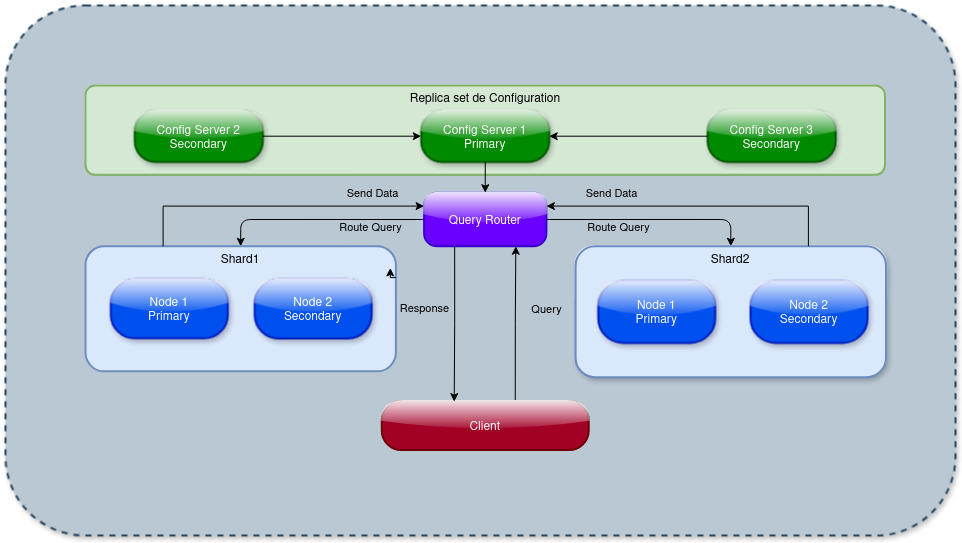
\includegraphics[width=0.8\textwidth]{architectures/MongoDBShards.jpg}
    \caption{Impact de l'indexation sur les performances.}
    \label{fig:indexation}
\end{figure}
\section{Réplication et Sharding}
\begin{figure}[H]
    \centering
    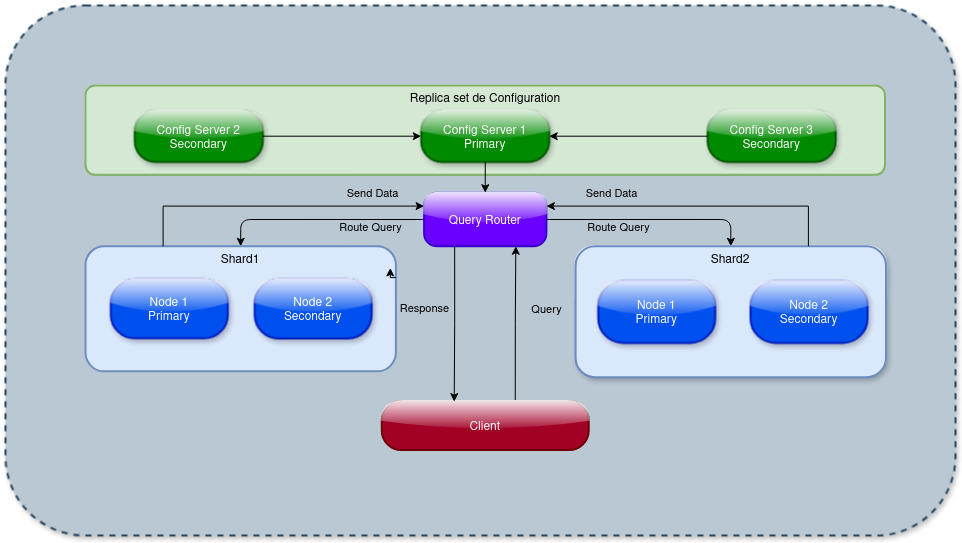
\includegraphics[width=0.8\textwidth]{architectures/MongoDBShards.jpg}
    \caption{Impact de la réplication et du sharding sur les performances.}
    \label{fig:replication_sharding}
\end{figure}

\chapter{Analyse des Résultats}
\section{Performances des Requêtes}
\begin{itemize}
	\item MongoDB excelle pour les lectures non indexées et les mises à jour fréquentes de la structure des données.
	\item MySQL est plus performant pour les requêtes transactionnelles complexes et les lectures indexées.
	\item L'indexation est un facteur clé pour améliorer les performances des requêtes.
	\item Les performances de MongoDB augmentent grandement avec l'indexation.
	\item MySQL est plus rapide pour les requêtes indexées.
	\item Les performances de MongoDB sont meilleures pour les lectures non indexées.
	\item L'indexation est un facteur clé pour améliorer les performances des requêtes.
\end{itemize}
\section{Impact de la Réplication et du Sharding}
\begin{itemize}
	\item La réplication et le sharding améliorent la tolérance aux pannes et la scalabilité.
	\item La réplication augmente la latence d'écriture, mais garantit une haute disponibilité des données.
	\item Le sharding améliore les performances des lectures et écritures parallèles.
	\item MySQL Cluster offre des fonctionnalités similaires à MongoDB, mais avec une configuration plus complexe.
	\item MongoDB est plus adapté pour les applications nécessitant une scalabilité horizontale et une haute disponibilité.
\end{itemize}
\section{Critique des résultats}

\begin{itemize}
	\item Les tests ont été réalisés sur des configurations de base, sans optimisations spécifiques.
	\item Les performances peuvent varier en fonction de la charge, de la volumétrie des données, et de la configuration matérielle.
	\item Les résultats sont indicatifs et doivent être confirmés par des tests plus approfondis.
	\item Les performances des SGBD dépendent fortement de la nature des requêtes et de la structure des données.
	\item Les tests ont été réalisés sur des scénarios simples, mais les performances peuvent varier dans des cas d'utilisation réels.
\end{itemize}

\chapter{Conclusion}
Cette étude met en évidence les avantages et inconvénients des architectures NoSQL et relationnelles dans divers scénarios. MongoDB offre une grande flexibilité et scalabilité, tandis que MySQL reste performant pour des cas nécessitant des transactions complexes.

\end{document}